\documentclass{report}
\usepackage{graphicx}
\usepackage{amsmath}
\usepackage{indentfirst}
 
\begin{document}
 
 \begin{titlepage}
	\centering
    
\includegraphics[width=4cm, height=3cm]{head-white-gray-big.png}

	{\scshape\LARGE Washington State University \par}
	\vspace{1cm}
	{\scshape\Large Computer Science 322\par}
	\vspace{1.5cm}
	{\huge\bfseries Design Specification\par}
	\vspace{2cm}
	{\Large\itshape David Harkins\par}
	\vfill
	Instructor\par
	\textsc{Neil Corrigan}

	\vfill
	{\large \today\par}
\end{titlepage}
\pagebreak
 
\tableofcontents{}
\pagebreak

\listoffigures

\section*{Revision History}

\begin{description}
\item[Revision 2, \today]: Updated based on the notes provided from the initial draft.
\item[Revision 1, April 1, 2016]: The initial version of the design specification.
\end{description} 
\pagebreak



\iffalse Section 1: Introduction ---------------------------- \fi
\chapter{Introduction}
 	The purpose this document is to create a design of the Turing machine simulation program. This document will be used by the developers that will be doing the implementing. With each developer having a copy of this design they will be able to work largely independently. This will increase the amount of developers that can be working on this project at a single time. It will also provide a single uniform guide so each developer is working towards the same common goal.
    
    This design document will provide and explain the design of the Turing machine simulation program. First, this will be a class diagram, made with the unified modeling language, that will be used to specify the classes and their relationships. Next, each class will be described in more detail without using UML. Each class description will have a short description, the associations to other classes, the attributes, and the methods. 
    The next thing will that will be described is the commands. Each command design will provide a description, examples of output, how to call it, and if there are any limitations of when it can be called.
  
    

\iffalse Section 2: Architecture ---------------------------- \fi
\chapter{Architecture}


\begin{figure}[!ht]
  	\centering
	\
    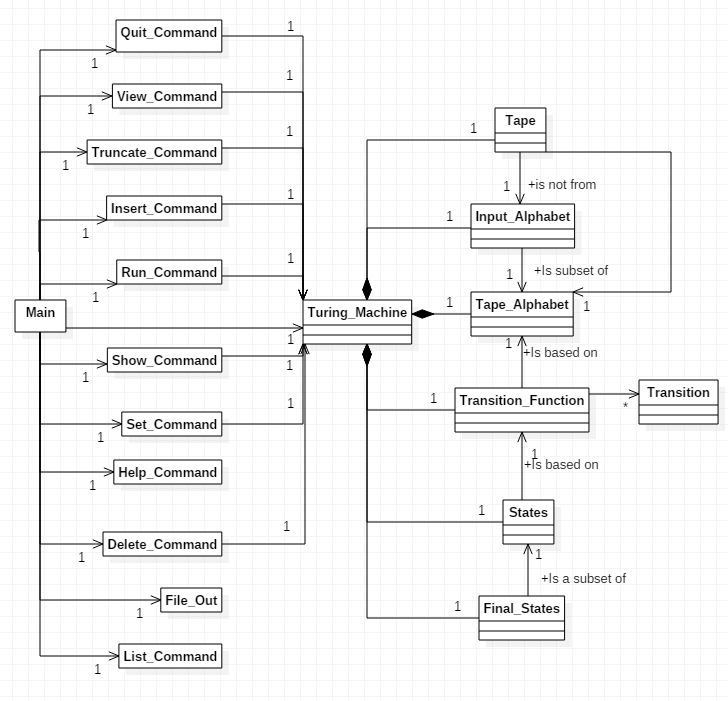
\includegraphics[width=1\textwidth]{UML_Overview.png}
  \caption{The associations between the classes.}
\end{figure}

\begin{figure}[!ht]
  	\centering
	\
    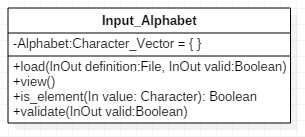
\includegraphics[scale=0.90]{Input_Alphabet.png}
  \caption{Input\_Alphabet class diagram.}
\end{figure}

\begin{figure}[!ht]
  	\centering
	\
    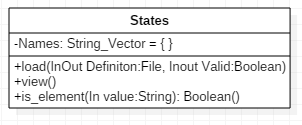
\includegraphics[scale=0.90]{States.png}
  \caption{States class diagram.}
\end{figure}

\begin{figure}[!ht]
  	\centering
	\
    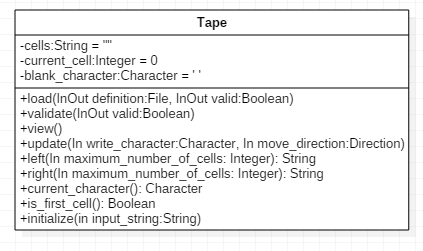
\includegraphics[scale=0.90]{Tape.png}
  \caption{Tape class diagram.}
\end{figure}

\begin{figure}[!ht]
  	\centering
	\
    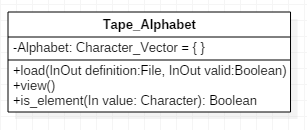
\includegraphics[scale=0.90]{Tape_Alphabet.png}
  \caption{Tape\_Alphabet class diagram.}
\end{figure}

\begin{figure}[!ht]
  	\centering
	\
    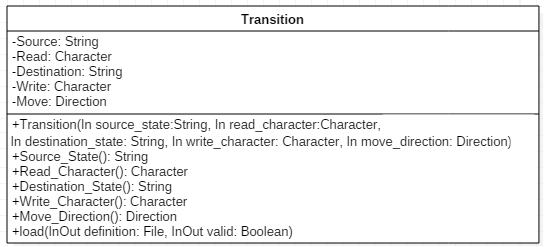
\includegraphics[scale=0.90]{Transition_v2.png}
  \caption{Transition class diagram.}
\end{figure}

\begin{figure}[!ht]
  	\centering
	\
    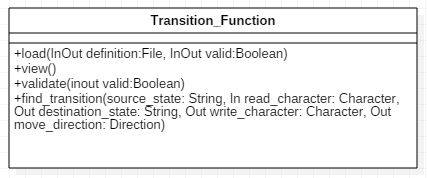
\includegraphics[scale=0.90]{Transition_Function.png}
  \caption{Transition\_Function class diagram.}
\end{figure}

\begin{figure}[!ht]
  	\centering
	\
    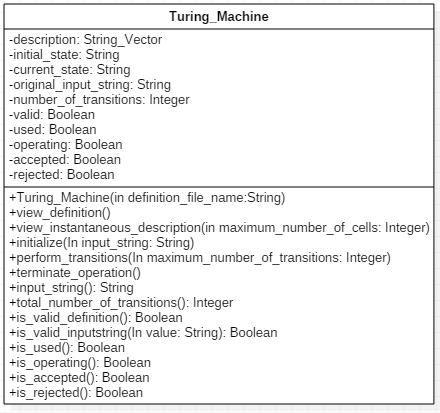
\includegraphics[scale=0.90]{Turing_Machine.png} 
  \caption{Turing\_Machine class diagram.}
\end{figure}

\begin{figure}[!ht]
  	\centering
	\
    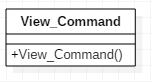
\includegraphics[scale=0.90]{View_Command.png}
  \caption{View\_Command class diagram.}
\end{figure}

\begin{figure}[!ht]
  	\centering
	\
    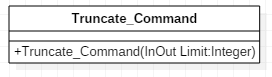
\includegraphics[scale=0.90]{Truncate_Command.png}
  \caption{Truncate\_Command class diagram.}
\end{figure}

\begin{figure}[!ht]
  	\centering
	\
    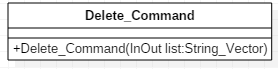
\includegraphics[scale=0.90]{Delete_Command.png}
  \caption{Delete\_Command class diagram.}
\end{figure}

\begin{figure}[!ht]
  	\centering
	\
    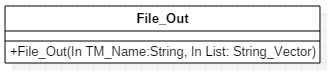
\includegraphics[scale=0.90]{File_Out.png}
  \caption{File\_Out class diagram.}
\end{figure}

\begin{figure}[!ht]
  	\centering
	\
    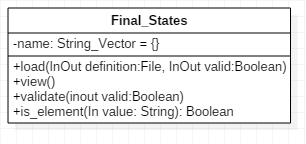
\includegraphics[scale=0.90]{Final_States.png}
  \caption{Final\_States class diagram.}
\end{figure}

\begin{figure}[!ht]
  	\centering
	\
    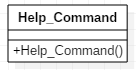
\includegraphics[scale=0.90]{Help_Command.png}
  \caption{Help\_Command class diagram.}
\end{figure}


\begin{figure}[!ht]
  	\centering
	\
    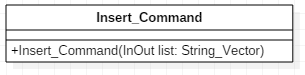
\includegraphics[scale=0.90]{Insert_Command.png}
  \caption{Insert\_Command class diagram.}
\end{figure}

\begin{figure}[!ht]
  	\centering
	\
    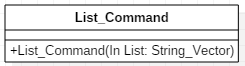
\includegraphics[scale=0.90]{List_Command.png}
  \caption{List\_Command class diagram.}
\end{figure}

\begin{figure}[!ht]
  	\centering
	\
    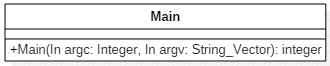
\includegraphics[scale=0.90]{Main.png}
  \caption{Main class diagram.}
\end{figure}

\begin{figure}[!ht]
  	\centering
	\
    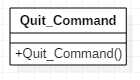
\includegraphics[scale=0.90]{Quit_Command.png}
  \caption{Quit\_Command class diagram.}
\end{figure}

\clearpage

\begin{figure}[!ht]
  	\centering
	\
    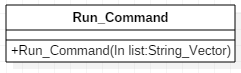
\includegraphics[scale=0.90]{Run_Command.png}
  \caption{Run\_Command class diagram.}
\end{figure}

\begin{figure}[!ht]
  	\centering
	\
    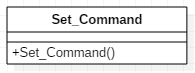
\includegraphics[scale=0.90]{Set_Command.png}
  \caption{Set\_Command class diagram.}
\end{figure}

\begin{figure}[!ht]
  	\centering
	\
    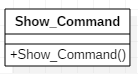
\includegraphics[scale=0.90]{Show_Command.png}
  \caption{Show\_Command class diagram.}
\end{figure}


\iffalse Section 3: Data Dictionary ---------------------------- \fi
\chapter{Data Dictionary}

    \section{Turing\_Machine}
	\subsection{Description}
    
    The Turing\_Machine class is used to control the simulation of a Turing Machine. It is composed of the elements required to run a Turing machine and it handles the interaction between them.
    
    \subsection{Associations} 
    The class Turing\_Machine is composed of a single one of each of the following; Tape, Input\_Alphabet, Transition\_Function, States, and Final\_States.
    \subsection{Attributes} 
    
      \subsubsection{ description: String\_Vector }
      The attribute description stores the description that was loaded from the Turing Machine definition file.
      
      \subsubsection{ initial\_state: String }
      The attribute the initial\_state of the Turing machine that was loaded from the Turing Machine definition file.
      
      \subsubsection{ current\_state: String  }
      The attribute the current\_state that the Turing machine is on in the simulation.
      
      \subsubsection{ original\_input\_string: String }
      The attribute original\_input\_string contains the original input string that was initially put on the Turing Machine tape.
      
      \subsubsection{ number\_of\_transitions:Integer  }
      This attribute stores the number of transitions that the Turing Machine has run.
      
      \subsubsection{ valid: Boolean  }
      This attribute holds the state for if the Turing\_Machine is a valid Turing Machine.
      
      \subsubsection{ used: Boolean }
      This attribute stores if the Turing\_Machine has been used before.
      
      \subsubsection{ operating: Boolean  }
      This attribute stores if the Turing\_Machine is currently operating on a input string.
      
      \subsubsection{ accepted: Boolean  }
      This attribute stores if the Turing\_Machine has accepted the input string,
      
      \subsubsection{ rejected: Boolean  }
      The attribute rejected is used to store if the Turing\_Machine was rejected or not.
    
     \subsection{Methods} 
    
     \subsubsection{ Turing\_Machine(In definition\_file\_name:String)  }
     This function accepts a file name and appends ".TM" to it and attempts to load the file. If it is unable to load the file it displays an error and returns. If the file is found and is able to be read, this function will read the name of the description of the Turing Machine from the file, and the open file will be passed to the following classes in this order. First States, Input\_Alphabet, Tape\_Alphabet, Transition\_Function, back to this function where it will read the initial state and pass the file to Tape\_Alphabet, and finally to Final\_States.
     
     \subsubsection{ view\_definition()  }
     This function prints out the definition of the Turing Machine that was loaded from the Turing Machine definition file. To do this the function calls the correct display function for each component contained within it.
     
     
     \subsubsection{ view\_instantaneous\_description(in maximum\_number\_of\_cells: Integer)  }
     This function displays the instantaneous description to the user. When displaying the max number of cells to display on each side that are displayed is limited to the maximum\_number\_of\_cells that is passed as a parameter.  
     
     
     \subsubsection{ initialize(In input\_string:String  }
     This function sets the current input string to input\_string if operating is set to false. Next, the initial state of the Turing Machine's tape is displayed to the user. If operating is set to true, an error message is displayed and the function returns.
     
     \subsubsection{ perform\_transitions(In maximum\_number\_of\_transitions: Integer)  }
     This function call will simulate the Turing Machine that is loaded in from the Turing Machine definition file on the set input string. The simulation can only happen if operating is set to true, accepted and rejected are both set to false. The function will continue to simulate the Turing Machine until the amount of transitions reaches the maximum\_number\_of\_transitons unless the Turing machine rejects or accepts the input string before the maximum\_number\_of\_transitions is met. If the Turing Machine is accepted or rejected, operating is set to false, and a message is displayed to the user.
     
     \subsubsection{ terminate\_operation()  }
     This function stops the operation on the current input string by setting the operating variable to false. This makes the Turing\_Machine unable to continue and forces the user to start a new simulation on a input string.
     \subsubsection{ input\_string(): String  }     
     This function returns the current input string that the Turing\_Machine is operating on.
     \subsubsection{ total\_number\_of\_transitions(): Integer  }
     This function returns the amount of transitions that have been completed on the currently selected input string.
     
     \subsubsection{ is\_valid\_inputstring(In value:String)}
     This function returns if the input string is valid. This function checks that every character in the input string is contained within the input\_alphabet. If any character contains a character that is reserved or is not in the input\_alphabet it returns false. If it contains only characters that are in the input alphabet it returns true.   
     
     
     \subsubsection{ is\_valid\_definition(): Boolean  }
     This function returns if the validation by the components, that are contained within the Turing\_Machine class, all validated correctly.
     \subsubsection{ is\_used(): Boolean  }      
     This function returns if the Turing\_Machine has been used before.
     \subsubsection{ is\_operating(): Boolean  } 
     This function returns the value of operating.
     \subsubsection{ is\_accepted(): Boolean  }
     This function returns the value of accepted.
     \subsubsection{ is\_rejected(): Boolean  }
     This function returns the value of rejected.

    
    
    
    
\section{Tape}
	\subsection{Description}
    The tape of a Turing machine consists of an ordered sequence of cells, indexed starting at 0, which may grow to any size needed up to the limit of storage during operation of the machine on an input string. Each cell contains a character in the tape alphabet. An input string is stored in the lowest numbered tape cells at the beginning of operation, and all other tape cells initially contain the blank character. The current cell starts at the first cell on the tape. In performing a transition of the Turing machine, the character contained in the current cell may be read and written, and the current cell may be moved one cell to the left or right. The tape exists only as part of a Turing machine.
    \subsection{Associations} 
    The class Tape is a component of the class Turing\_Machine, receiving messages delegated to it by the Turing machine.
    The association not filled with the class Input\_Alphabet used to validate that the blank character for initialization and extension of the Turing machine tape is in the tape alphabet.
    \subsection{Attributes} 
    \subsubsection{ cells:String = "" }
    The attribute cells is a dynamically growing character string containing the Turing machine tape. In preforming an update, the tape may be extended by appending a blank character.
    
    \subsubsection{ current\_cell:Integer = 0 }
    The index of the current cell on the Turing machine tape is stored in the attribute current\_cell.
    
    \subsubsection{blank\_character:Character = ' ' }
    The blank character used, to initialize and extend the Turing machine tape, is contained in the attribute blank\_character.
    \subsection{Methods} 
    
    \subsubsection{load(InOut definition:File, InOut valid:Boolean)}
    The method load reads the blank character from the Turing machine definition file. If the blank character is reserved or not printable, or the next keyword does not follow it in the file, an error message is displayed and valid is set to false.
    
    \subsubsection{validate(InOut:Boolean)}
    The method validate determines if the blank character of the Turing machine is in the tape alphabet, but not in the input alphabet. If the blank character is in the input alphabet, or is not in the tape alphabet, an error message is displayed and valid is set to of false.
    
    \subsubsection{view()}
    The method view displays the blank character of the Turing machine.
    
    \subsubsection{initialize(In input\_string:String)}
    The method initialize sets the Turing machine tape to the input string followed by a blank character, replacing the previous contents of the tape. The current cell is set to the first cell on the tape, indicated by the index 0.
    
    \subsubsection{update(In write\_character:Character, In move\_direction:Direction)}
    The method update first determines if the update of the Turing machine tape is possible. The method returns if a left move is specified from the first cell. If a right move is specified from the last cell, a blank character is appended to the tape. Assuming that the update may be performed, the character to write on the tape is stored in the current cell, replacing the previous character in that cell. To move the current cell one cell to the left, the index is decremented, or to move the current cell one cell to the right, the index is incremented. 
    
    \subsubsection{left(In maximum\_number\_of\_cells:Integer):String}
    
    The method left returns a character string up to the maximum number of cells from the Turing machine tape to the left of the current cell, excluding that cell. The length of the string will be less than the maximum if there are fewer cells to the left of the current cell. If the string is truncated from the tape, the reserved character '<' will be added to the beginning of the string.
    
    \subsubsection{right(in maximum\_number\_of\_cells:Integer):String }
    The method right returns a character string up to the maximum number of cells from the Turing machine tape to the right of the current cell, including that cell. The length of the string will be less than the maximum if there are fewer cells to the right of the current cell up to the rightmost nonblank character. If the string is truncated from the tape, the reserved character '>' will be added to the end of the string.
    
    \subsubsection{ current\_character():Character}
    
    The method current\_character returns the character contained in the current cell on the Turing machine tape.
    
    \subsubsection{is\_first\_cell():Boolean}
    
    The method is\_first\_cell returns a value of true if the current cell on the Turing machine tape is the first cell, indicated by the index 0. Otherwise, it returns a value of false.
    
    
    
    
    
    
    
      \section{Input\_Alphabet}
	\subsection{Description}
    	The list of characters that are allow for the user to enter. This must be a subset of the Tape\_Alphabet.
        The association is class Tape is not from Input\_Alphabet, the
    \subsection{Associations}
    This class is a component of the class Turing\_Machine, receiving messages delegated to it by the Turing machine.
        
    \subsection{Attributes} 
    
    \subsubsection{Alphabet:Character\_Vector = \{ \}}
    This attribute is used to store the list of Input\_Alphabet characters that were loaded from the Turing Machine definition file. The characters contained must be a subset of the ones contained in the Tape\_Alphabet and also does not include the blank character.
    
    \subsection{Methods} 
    \subsubsection{load(InOut definition:File, InOut valid:Boolean)}
    This function attempts to load the Input\_Alphabet from the File. If there is a failure on reading or parsing the file, the function will set valid to false, display the error, and return. If the function is able to read and parse the file, the function will return.
    
    \subsubsection{view()}
    This function displays the contents of Alphabet.
    
    \subsubsection{is\_element(In value: Character): Boolean}
    This function checks if the parameters character is contained within Alphabet.
    
    \subsubsection{validate(InOut valid:Boolean)}
    This function compares the elements loaded from the Turing Machine definition file to the ones in Input\_Alphabet
    
    
    
    
    
      \section{Tape\_Alphabet}
	\subsection{Description}
    The list of characters that can be written to the type cells in Tape. 
    \subsection{Associations} 
     This class is a component of the class Turing\_Machine, receiving messages delegated to it by the Turing machine.
    \subsection{Attributes} 
    \subsubsection{Alphabet: Character\_Vector = \{\}}
    The attribute Alphabet is used to store the characters that can be placed on the tape cells.
    \subsection{Methods} 
    \subsubsection{load(InOut definition:File, InOut valid:Boolean)}
    This method is used to load new Tape\_Alhpabet characters from a file. This stops when a keyword is found or the end of the file is reached. All errors will be displayed to the user. If there are any errors the function will set valid to fail thereby rejecting the Turing Machine Definition file. 
    
    
    \subsubsection{is\_element(In value: Character): Boolean}
    This method is used to check if the character is within the alphabet. 
    
    
    
      \section{Transition\_Function}
	\subsection{Description}
    The transition function is responsible providing easy access to the class Transition from other classes. It is responsible for loading the transitions, selecting the correct one for the next transition if available, validating the transitions, and printing out the transitions.
    \subsection{Associations} 
     This class is a component of the class Turing\_Machine, receiving messages delegated to it by the Turing machine.
     This class has a is based on association with the class States.
    \subsection{Attributes} 
    None.
    \subsection{Methods} 
      \subsubsection{load(InOut definition:File, InOut valid:Boolean)}
      This method is passed a File and it reads it until, it finds the next section's tag, a error in parsing the data happens, or it reaches the end of the file.
      \subsubsection{view()}
      	This method is used to print out the value of the transition. This is used by class Show\_Command though the class Turing\_Machine.
      \subsubsection{validate(InOut valid:Boolean)}
      This method is used to validate the transitions. It checks that each transition is based on the class States.
      \subsubsection{find\_transition(source\_state:String, In read\_character: Character, Out destination\_state: String, Out write\_character: Character, Out move\_direction: Direction)}
      This method searches all of the class transition until it: finds a matching source and read character; or it searched all of the Transitions and was unable to find one. If the class transition\_Function is able to find a Transition that matches it will return the Transition. If the class Transition\_Function is unable to find a transition that matches it returns an error.
    
    
      \section{Transition}
	\subsection{Description}
    This class is designed to hold a single Turing Machine definition transition. All other classes that want to use it must access it by using the class Transition\_Function.
    
    \subsection{Associations} 
     This class has one to many association with the class Transition\_Function.  
    \subsection{Attributes} 

	\subsubsection{Source: String}
    This attribute contains the name of the current state that the Turing machine must be in to use this transition.
    \subsubsection{Read: Character}
    This attribute contains the name of the state that is currently the current tape cell.
    \subsubsection{Destination: String}
    This attribute contains the name of the state that the Turing Machine will transfer to if it uses this transition.
    \subsubsection{Write: Character}
    This attribute contains the character that will be written to the class Tape where the Turing Machine is currently pointing. This happens before the transition moves the current\_cell that is contained in the class Tape.
    \subsubsection{Move:Direction}
    This attribute contains the direction that the tape head will move after the character is written to the class Tape. It can only be to the right or to the left.
    
    \subsection{Methods} 
      \subsubsection{load(InOut definition:File, InOut valid:Boolean)}
      This method is used to load the Transitions from the Turing Machine definition file. The method will stop searching the file a new keyword or the end of the file. It displays any errors out to the user.
        \subsubsection{Transition(In source\_state:String, In read\_character:Character, In destination\_state: String, In write\_character: Character, In move\_direction: Direction)}
        
    
    \subsubsection{Source\_State():String}
    This method is used to get the current value of Source attribute that is contained in the class Transition.
    \subsubsection{Read\_Character(): Character}
    This method is used to get the current value of Read attribute that is contained in the class Transition.
    \subsubsection{Destination\_State(): String}
    This method is used to get the current value of State attribute that is contained in the class Transition
    \subsubsection{Write\_Character(): Character}
	This method is used to get the current value of write attribute that is contained in the class Transition
	\subsubsection{Move\_Direction(): Direction}
    This method is used to get the current value of Direction attribute that is contained in the class Transition.
    
    
\section{States}
	\subsection{Description}
    The possible states the Turing machine can be in at any given time.
    \subsection{Associations} 
     This class is a component of the class Turing\_Machine, receiving messages delegated to it by the Turing machine.
     The class Final\_States has an is a subset of association with the class States. 
    \subsection{Attributes} 
    \subsubsection{Names: String\_Vector =  \{ \}}
    This attribute contains all of the state names. They are loaded from a Turing Machine definition file and validated while they are loaded.
    
    \subsection{Methods} 
    
      \subsubsection{load(InOut definition:File, InOut valid:Boolean)}
      This method is called by the Turing\_Machine class that it is contained inside. This method will attempt to load Turing Machine states from the file until when a keyword is found or the end of the file is reached. All errors will be displayed to the user. If there are any errors the function will set valid to fail thereby rejecting the Turing Machine Definition file. 
      
      
      
    \subsubsection{view()}
    	This method is used to display the current states that are attributes of the current class instance of States.
    \subsubsection{is\_element(In value:String): Boolean()}
    	This method is used to check if a state is contained in the current class instance of State.
    
    
    
    
    
      \section{Final\_States}
	\subsection{Description}
    The state that if the Turing Machine transitions into cannot leave, the Input String is accepted, and the class Turing\_machine sets operating to false.
    \subsection{Associations} 
     This class is a component of the class Turing\_Machine, receiving messages delegated to it by the Turing machine.
     This class has an is a subset of association with the class States.
    \subsection{Attributes} 
    \subsubsection{name: String\_Vector = \{ \}}
    This attribute contains all of the states that are considered final states. All of the Final\_States must be contained in the class States as well.
    \subsection{Methods} 
     \subsubsection{load(InOut definition:File, InOut valid:Boolean)}
     This method is called to load new final states into the class Final\_States. This stops when a keyword is found or the end of the file is reached. All errors will be displayed to the user. If there are any errors the function will set valid to fail thereby rejecting the Turing Machine Definition file. 
    \subsubsection{view()}
    This method is used to display all of the current final states in a formatting of the formal definition of the Turing Machine class.
    \subsubsection{validate(InOut valid:Boolean)}
    This method is used to make sure that each of the Final\_States in contained in the class States.
    \subsubsection{is\_element(In value String): Boolean)}
    This method is used to check if a state is a final state. The class Turing\_Machine uses this to check if the current transition is into a final state.
    
    
\section{Quit\_Command}
	\subsection{Description}
    When the Turing machine class is currently running on a input string the class the Quit\_Command will terminate the running on the input string. The Turing machine will neither accept or reject the input string is the Quit\_Command is used. If the command is used, and the Turing machine is not running on a input string, a error will be displayed, and Quit\_Command will return. 
    \subsection{Associations} 
    This class is associated with the class Main, receiving messages delegated to it by the user.
    The class Quit\_Command is associated with a single Turing\_Machine class.
    
    \subsection{Attributes} 
    None.
    
    \subsection{Methods} 
    \subsubsection{Quit\_Command()}
    The Quit\_Command function will terminate the running of a Turing machine on a input string. If there is no input string running or the Turing machine has accepted, rejected, or never been used before an error will be displayed and the function will return.
    
    
    
\section{View\_Command}
	\subsection{Description}
    The View\_Command displays the Turing machine definition file that is contained inside of a Turing machine. Before the function can be called, the program has insured that the Turing machine definition is valid.
    
    \subsection{Associations} 
    This class is associated with the class Main, receiving messages delegated to it by the user.
    
    The class View\_Command is associated with a single Turing\_Machine class.
    
    \subsection{Attributes}
    None.
    \subsection{Methods} 
    \subsubsection{View\_Command()}
    This function prints the currently stored Turing Machine definition from a Turing machine.    
    
    
\section{Truncate\_Command}
	\subsection{Description}
    The Truncate\_Command gets user input and updates the truncation setting. The value that the user enters must be an integer and greater than zero, if it is not an error, is displayed and the function returns without changing the setting. 
    \subsection{Associations}
    This class is associated with the class Main, receiving messages delegated to it by the user.
    
      The class Truncate\_Command is associated with a single Turing\_Machine class.
    
    \subsection{Attributes}
    None.
    \subsection{Methods} 
    \subsubsection{Truncate\_Command(InOut limit: Integer)}
    This function gets user input and updates the truncation setting. The value of the user input must be a integer and greater than zero. If it is not, an error message is displayed and the function returns without changing the setting. If the user enters nothing, the function returns without changing the setting or displaying any message.

    
\section{Insert\_Command}
	\subsection{Description}
    The class Insert\_Command allows the user to enter a new input string. The input string that will be  inserted can be used to run on the Turing Machine. If the user wishes to specify the empty string they must enter the backslash character. 
    \subsection{Associations} 
    This class is associated with the class Main, receiving messages delegated to it by the user.
    
      The class Insert\_Command is associated with a single Turing\_Machine class.
    
    \subsection{Attributes}
    None.
    \subsection{Methods} 
    \subsubsection{Insert\_Command(InOut list: String\_Vector)}
    This function will user input, and if the input is not empty, it will validate the input against the current Turing\_Machine. If the input is empty, the function will return with no display or change in list. If the input is invalid for the Turing Machine definition, an error is displayed and the function returns. If the input is valid, the new input string is added to the end of the list. If the user enters the backslash character will be replaced with an empty string before validation occurs.
    
    
      \section{Run\_Command}
	\subsection{Description}
    
    This class Run\_Command will start the Turing Machine running on a selected input string. 
    
\subsection{Associations} 
This class is associated with the class Main, receiving messages delegated to it by the user.
     The class Run\_Command is associated with a single Turing\_Machine class.
    \subsection{Attributes}
    None.
    \subsection{Methods} 
    \subsubsection{Run\_Command(In list:String\_Vector)}
    This function takes a list of input strings as a parameter and prompts for user input. The input that the function asks for is a number that is assigned to a input string. The number can be found using the list command on the command prompt. If the user enters nothing, the function will return without any message or without starting the Turing Machine. If the input is an invalid input string number, or the Turing Machine is already running on a input string, an error will be displayed, and the function will return. If the input is a valid string number, the input string that the user selected will be given to Turing\_Machine, and the function will return.
    
    
\section{Show\_Command}
	\subsection{Description}
    The show command lists the status of the program and Turing machine. The information displayed is based on user settings and the current status of the Turing Machine. The differences in the Turing machine status are: it has run before; is currently running; or was accepted; rejected or the user terminated it.
    \subsection{Associations} 
    This class is associated with the class Main, receiving messages delegated to it by the user.
      The class Show\_Command is associated with a single Turing\_Machine class.
    \subsection{Attributes}
    None.
    \subsection{Methods} 
    \subsubsection{Show\_Command()}
    The function Show\_Command() displays the status of the Turing Machine. The elements that are listed are the course name, semester, year, instructor, author, version number, max transitions, max cells to the left and right, the name of the Turing Machine file, and the Turing machine status. If the Turing machine has never been run before, a message is displayed to that effect. If the Turing machine is currently running, the input string it is running on is displayed as well as the number of transitions already preformed. If the Turing Machine has accepted, rejected, or the user has terminated operation, the number of transitions and reason the operation was stopped are displayed.    
    
    
    
\section{Set\_Command}
	\subsection{Description}
    This Set\_Command is used to change the maximum number of transitions for the Turing\_Machine to perform before the operation pauses.
    \subsection{Associations} 
    This class is associated with the class Main, receiving messages delegated to it by the user.
      The class Set\_Command is associated with a single Turing\_Machine class.
    
    \subsection{Attributes}
    None.
    \subsection{Methods}
    \subsubsection{Set\_Command()}
    This function displays the current setting of the maximum transitions and waits for user input. If the user enters nothing, the function returns without changing the setting or displaying a message. If the user does not enter a number greater than 0, and that is a integer, an error is displayed, and the function returns. If the input is valid, the maximum transitions is changed, a message is displayed, and the function returns.
    
    
    
    

\section{Help\_Command}
	\subsection{Description}
    This class Help\_Command displays the usage to the user. This displays all of the valid commands for the users to use and a short description of each.
    \subsection{Associations}   
    This class is associated with the class Main, receiving messages delegated to it by the user.
    \subsection{Attributes}
    None.
    \subsection{Methods} 
    \subsubsection{Help\_Command()}
    The Help\_Command displays the usage to the user.
    
    
    
    
\section{Delete\_Command}
	\subsection{Description}
    This class Delete\_Command is used to remove input strings from the input string list.
    \subsection{Associations} 
    This class is associated with the class Main, receiving messages delegated to it by the user.
      The class Delete\_Command is associated with a single Turing\_Machine class.
    
    \subsection{Attributes} 
    None.
    \subsection{Methods}
    \subsubsection{Delete\_Command(InOut list:String\_Vector)}
    This function prompts for the user to enter a valid input string index number. If the user enters nothing, the function returns without a message. If the user enters a number that is not above zero, or that is not a integer, an error is displayed and the function returns. If the user enters a valid input string, index it is deleted, a message is displayed, and the function returns.
    
    
    
    
    
\section{File\_Out}
	\subsection{Description}
    This class File\_Out is used to offload the input string list when the application is closing. The file will only be written out to disk if there were changes made to the file (Invalid input string was removed, the user added a string, or user deleted a string). 
    \subsection{Associations}
    This class is associated with the class Main, being called when the application terminates.
    \subsection{Attributes}
    None.
    \subsection{Methods} 
    \subsubsection{File\_Out(In TM\_Name:String, In List:String\_Vector)}
    This function saves the entire input string list a file named after the parameter TM\_Name. This will overwrite the original input string list if it exists, or will create a new one if it does not. If it is unable to save the input string file to disk, an error will be displayed, and the application will terminate. If the function was able to save the file to disk, a message is displayed and the application terminates.    
    
    
    
    
    
    
\section{List\_Command}
	\subsection{Description}
    	This class List\_Command displays the current list of input strings to the user. If there are no input strings a message will be displayed saying such.
    
    \subsection{Associations} 
    This class is associated with the class Main, receiving messages delegated to it by the user.
    \subsection{Attributes}
    None.
    \subsection{Methods} 
    \subsubsection{List\_Command(In List: String\_Vector)}
    This function displays each input string on its own line with its input string index before it, and the function returns. If there are no input strings a message is displayed saying such and the function returns.
    




\section{Main}
	\subsection{Description}
    This class Main is the top level entry point for the application. It is in control of starting all of the other classes.
    \subsection{Associations} 
      The class Main is associated with a single Turing\_Machine class, a single Quit\_Command, a single View\_Command, a single Truncate\_Command, a single Insert\_command, a single Run\_Comannd, a single Show\_Command, a single Set\_Command, a single Help\_Command, a single Delete\_Command, a single File\_Out, and a single List\_Command.
    
    \subsection{Attributes}
    None.
    \subsection{Methods} 
    \subsubsection{Main(argc: integer, argv: String\_Vector): integer}
    This function attempts to load the Turing Machine definition file named after the user passed parameter. If the Turing Machine file is able to be loaded, and it is valid, the function continues. If it was not able to be loaded, or it was invalid, an error message is displayed, and the application terminates. Next, the function attempts to load the input string file. On failure or success, the application continues to a loops that prompts for a command from the user, and calls the correct function to handle it.


    

    
    
\iffalse Section 4: User Interface ---------------------------- \fi
\chapter{User Interface}
     \section{Command Line Invocation}
     
     \subsubsection{Command line invocation with a valid file}
     \begin{verbatim}
Example of running the application with a command line argument (Normal):

$ TM Definition
Turing successfully loaded.
Command:
	\end{verbatim}
    
     \subsubsection{Command line invocation with a invalid file}
     \begin{verbatim}
Example of running the application with a command line argument (Error):

$ TM Definition_error
Error unable to load Turing Machine definition file.
$
	\end{verbatim}
     
     \section{Help Command}
     \begin{verbatim}
      Example of using the help command:

      Command: h

      (D)elete   - Delete input string from list.
      E(x)it     - Exit application.
      (H)elp     - Help user.
      (I)nsert   - Insert input string into list.
      (L)ist     - List input strings.
      (Q)uit     - Quit operation of Turing machine on input string. 
      (R)un      - Run Turing machine on input string.
      S(e)t      - Set maximum number of transitions to perform. 
      Sho(w)     - Show status of application.
      (T)runcate - Truncate instantaneous description.
      (V)iew     - View Turing machine.

      Command: 
      \end{verbatim}
      \pagebreak
     \section{Show Command}
     
     \begin{verbatim}
Example of using the show command:

Command: w

Course name: CPT_S 322
Semester: Spring
Year: 2016

Instructor: Neil Corrigan
Author: David Harkins

Version number: 1
Max transitions: 10
Max cells to left and right: 10
Name of TM: A
TM Status: Completed
The input string aaabb has been accepted in 7 transitions.
    
Command: 
\end{verbatim}
     
     
     \section{View Command}
     The view command is used to view the currently loaded Turing machine definition file.

\begin{verbatim}
Example of using the view command:

Command: v

This Turing machine accepts the language 
of one or more a's followed by the same number of b's.

Q = {s0, s1, s2, s4}
	
Sigma = {a, b}

Gamma = {a, b, X, Y, -}

Delta(s0, a) = (s1, X, R)
Delta(s0, Y) = (s3, Y, R)
Delta(s1, a) = (s1, a, R)
Delta(s1, b) = (s2, Y, R)
Delta(s1, Y) = (s1, Y, R)
Delta(s2, a) = (s2, a, R)
Delta(s2, X) = (s0, X, R)
Delta(s2, Y) = (s2, Y, R)
Delta(s3, Y) = (s3, Y, R)
Delta(s3, -) = (s4, -, R)

Q0 = s0

B = -

F = {s4}


Command: 
\end{verbatim}
     \section{List Command}
     \begin{verbatim}
Example of using the list command:

Command: l

1. a
2. ab
3. \
4. aaabb
5. aaaaaaaaaaabbbbbbbbbb
6. aabb
7. aaaaaabbbbbbb
8. ba
9. aba
10. bb

Command: 
\end{verbatim}
     \section{Insert Command}
\begin{verbatim}
Example of using insert command:

Command: i

Input string: abbb
String inserted into list!
    
Command: 
\end{verbatim}     
     \section{Delete Command}
     \subsubsection{Delete command with a valid input string index}
     \begin{verbatim}
Example of using the delete command (Normal):

Command: d

Input string number: 1
String deleted!

Command: 
\end{verbatim}

\subsubsection{Delete command with a invalid input string index}
\begin{verbatim}
Example of using the delete command (Error):

Command: d

Input string number: -1
Unable to delete, invalid input string index.

Command: 
\end{verbatim}


     \section{Set Command}
     
\subsubsection{The set command with valid input.}
\begin{verbatim}
Example of using the set transition command (Normally):

Command: e

Maximum number of transitions [1]: 20
Number of transitions changed to 20.
    
Command: 
\end{verbatim}

\subsubsection{The set command with invalid input.}
\begin{verbatim}
Example of using the set transition command (With error):

Command: e

Maximum number of transitions [1]: -1
Error, unable to change transitions. The new value must be greater or equal to 1
    
Command: 
\end{verbatim}
     
     \section{Truncate Command}
     
\subsubsection{The truncate command with valid input}
     \begin{verbatim}
Example of using the truncate command (Normal):

Command: t

Maximum number of cells [32]: 10
Setting changed!
    
Command: 
\end{verbatim}

\subsubsection{The truncate command with invalid input}
\begin{verbatim}
Example of using the truncate command (Error):

Command: t

Maximum number of cells [32]: -1
Error, unable to change max cells. The new value must be greater or equal to 1
    
Command: 
\end{verbatim}
     
     \section{Run Command}
\subsubsection{Using the run command with a valid string input index number}
     \begin{verbatim}
Example of using the run command (Normal):

Command: r

Input string number: 1
0. [s0]aaabb
7. XXXXY-[s4]
Input string aaabb was accepted in 7 transitions.

Command: 
\end{verbatim}

\subsubsection{Using the run command with a invalid string input index number}
\begin{verbatim}
Example of using the run command (Error):

Command: r

Input string number: -1
Invalid input string index.

Command: 
\end{verbatim}


     \section{Quit Command}
\subsubsection{Quit command running on input string}
     \begin{verbatim}
Example of using the quit command (Normal):

Command: q

Input string aaabb was not accepted or rejected in 112 transitions.

Command: 
\end{verbatim}

\subsubsection{Attempt to Quit on a Turing machine not running on a input string}
     \begin{verbatim}
Example of using the quit command (Error):

Command: q

Unable to stop running on input string because Turing machine 
was not running on input string.

Command: 
\end{verbatim}

\pagebreak
     \section{Exit Command}
     
\subsubsection{Exit command with save normally.}
     \begin{verbatim}
Example of using the exit command (Normal):

Command: x

Input string file successfully saved to disc.

$ 
\end{verbatim}

\subsubsection{Exit command with save Error.}
     \begin{verbatim}
Example of using the exit command (Error):

Command: x

Input string file was unable to be saved to disc.

$ 
\end{verbatim}
     
    
\iffalse Section 5: File ---------------------------- \fi
\chapter{File} 	
    
\section{Turing Machine Definition File} 
The following is an example of the Turing machine file format.

\begin{verbatim}
Example of using the view command:

Command: v

This Turing machine accepts the language 
of one or more a's followed by the same number of b's.

STATES: = s0 s1 s2 s4
	
INPUT_ALPHABET: = a b

TAPE_ALPHABET: = a b X Y -

TRANSITION_FUNCTION:
s0 a  s1 X R
s0 Y  s3 Y R
s1 a  s1 a R
s1 b  s2 Y R
s1 Y  s1 Y R
s2 a  s2 a R
s2 X  s0 X R
s2 Y  s2 Y R
s3 Y  s3 Y R
s3 -  s4 - R

INITIAL_STATE: = s0

BLANK_CHARACTER: = -

FINAL_STATES: s4


Command: 
\end{verbatim}


\section{Input String File} 

The following is an example of the input string file format.
\begin{verbatim}
a
ab
\
aaabb
aaaaaaaaaaabbbbbbbbbb
aabb
aaaaaabbbbbbb
ba
aba
bb
\end{verbatim}
   
  

\iffalse Section References: ---------------------------- \fi
\chapter{References}

\begin{itemize}
\item Neil Corrigan - General notes, lecture and help.
\end{itemize}

 

 
\end{document}

